% Generated by paper/scripts/writing_sample_exhibits.py.
\begin{figure}[H]
\centering
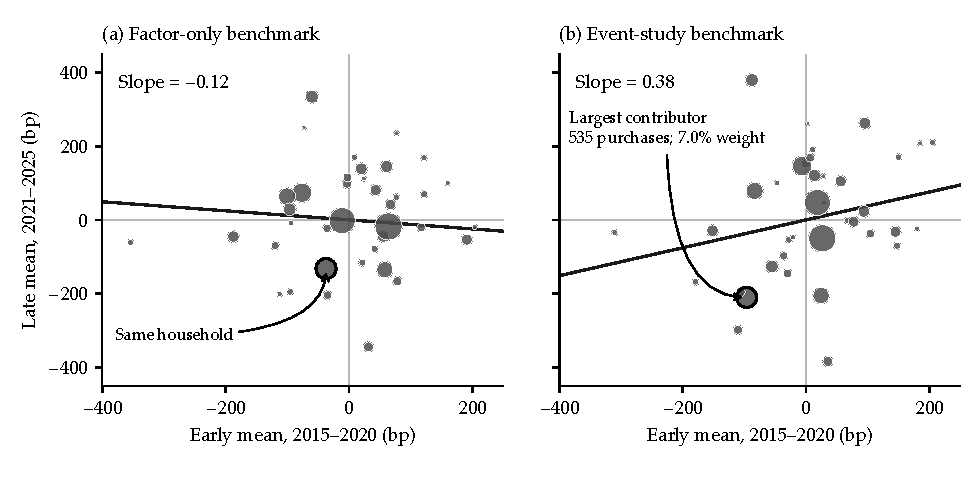
\includegraphics[width=\textwidth]{figures/writing_sample_households.pdf}
\caption{Household purchase returns in 2015--2020 and 2021--2025 under two benchmarks. Each point represents one of the 38 households in the persistence sample. Both panels use the same 7,964 purchases, and each period's means are residuals from a weighted regression on early trading activity. Point area is proportional to the geometric-mean weight, and lines are weighted regression fits with the slopes of Table~\ref{tab:tau}. The labeled household has negative residual means in both periods under both benchmarks and makes the largest contribution to the event-study covariance.}
\label{fig:benchmark-persistence}
\end{figure}
